\documentclass[1p]{elsarticle_modified}
%\bibliographystyle{elsarticle-num}

%\usepackage[colorlinks]{hyperref}
%\usepackage{abbrmath_seonhwa} %\Abb, \Ascr, \Acal ,\Abf, \Afrak
\usepackage{amsfonts}
\usepackage{amssymb}
\usepackage{amsmath}
\usepackage{amsthm}
\usepackage{scalefnt}
\usepackage{amsbsy}
\usepackage{kotex}
\usepackage{caption}
\usepackage{subfig}
\usepackage{color}
\usepackage{graphicx}
\usepackage{xcolor} %% white, black, red, green, blue, cyan, magenta, yellow
\usepackage{float}
\usepackage{setspace}
\usepackage{hyperref}

\usepackage{tikz}
\usetikzlibrary{arrows}

\usepackage{multirow}
\usepackage{array} % fixed length table
\usepackage{hhline}

%%%%%%%%%%%%%%%%%%%%%
\makeatletter
\renewcommand*\env@matrix[1][\arraystretch]{%
	\edef\arraystretch{#1}%
	\hskip -\arraycolsep
	\let\@ifnextchar\new@ifnextchar
	\array{*\c@MaxMatrixCols c}}
\makeatother %https://tex.stackexchange.com/questions/14071/how-can-i-increase-the-line-spacing-in-a-matrix
%%%%%%%%%%%%%%%

\usepackage[normalem]{ulem}

\newcommand{\msout}[1]{\ifmmode\text{\sout{\ensuremath{#1}}}\else\sout{#1}\fi}
%SOURCE: \msout is \stkout macro in https://tex.stackexchange.com/questions/20609/strikeout-in-math-mode

\newcommand{\cancel}[1]{
	\ifmmode
	{\color{red}\msout{#1}}
	\else
	{\color{red}\sout{#1}}
	\fi
}

\newcommand{\add}[1]{
	{\color{blue}\uwave{#1}}
}

\newcommand{\replace}[2]{
	\ifmmode
	{\color{red}\msout{#1}}{\color{blue}\uwave{#2}}
	\else
	{\color{red}\sout{#1}}{\color{blue}\uwave{#2}}
	\fi
}

\newcommand{\Sol}{\mathcal{S}} %segment
\newcommand{\D}{D} %diagram
\newcommand{\A}{\mathcal{A}} %arc


%%%%%%%%%%%%%%%%%%%%%%%%%%%%%5 test

\def\sl{\operatorname{\textup{SL}}(2,\Cbb)}
\def\psl{\operatorname{\textup{PSL}}(2,\Cbb)}
\def\quan{\mkern 1mu \triangleright \mkern 1mu}

\theoremstyle{definition}
\newtheorem{thm}{Theorem}[section]
\newtheorem{prop}[thm]{Proposition}
\newtheorem{lem}[thm]{Lemma}
\newtheorem{ques}[thm]{Question}
\newtheorem{cor}[thm]{Corollary}
\newtheorem{defn}[thm]{Definition}
\newtheorem{exam}[thm]{Example}
\newtheorem{rmk}[thm]{Remark}
\newtheorem{alg}[thm]{Algorithm}

\newcommand{\I}{\sqrt{-1}}
\begin{document}

%\begin{frontmatter}
%
%\title{Boundary parabolic representations of knots up to 8 crossings}
%
%%% Group authors per affiliation:
%\author{Yunhi Cho} 
%\address{Department of Mathematics, University of Seoul, Seoul, Korea}
%\ead{yhcho@uos.ac.kr}
%
%
%\author{Seonhwa Kim} %\fnref{s_kim}}
%\address{Center for Geometry and Physics, Institute for Basic Science, Pohang, 37673, Korea}
%\ead{ryeona17@ibs.re.kr}
%
%\author{Hyuk Kim}
%\address{Department of Mathematical Sciences, Seoul National University, Seoul 08826, Korea}
%\ead{hyukkim@snu.ac.kr}
%
%\author{Seokbeom Yoon}
%\address{Department of Mathematical Sciences, Seoul National University, Seoul, 08826,  Korea}
%\ead{sbyoon15@snu.ac.kr}
%
%\begin{abstract}
%We find all boundary parabolic representation of knots up to 8 crossings.
%
%\end{abstract}
%\begin{keyword}
%    \MSC[2010] 57M25 
%\end{keyword}
%
%\end{frontmatter}

%\linenumbers
%\tableofcontents
%
\newcommand\colored[1]{\textcolor{white}{\rule[-0.35ex]{0.8em}{1.4ex}}\kern-0.8em\color{red} #1}%
%\newcommand\colored[1]{\textcolor{white}{ #1}\kern-2.17ex	\textcolor{white}{ #1}\kern-1.81ex	\textcolor{white}{ #1}\kern-2.15ex\color{red}#1	}

{\Large $\underline{12a_{0488}~(K12a_{0488})}$}

\setlength{\tabcolsep}{10pt}
\renewcommand{\arraystretch}{1.6}
\vspace{1cm}\begin{tabular}{m{100pt}>{\centering\arraybackslash}m{274pt}}
\multirow{5}{120pt}{
	\centering
	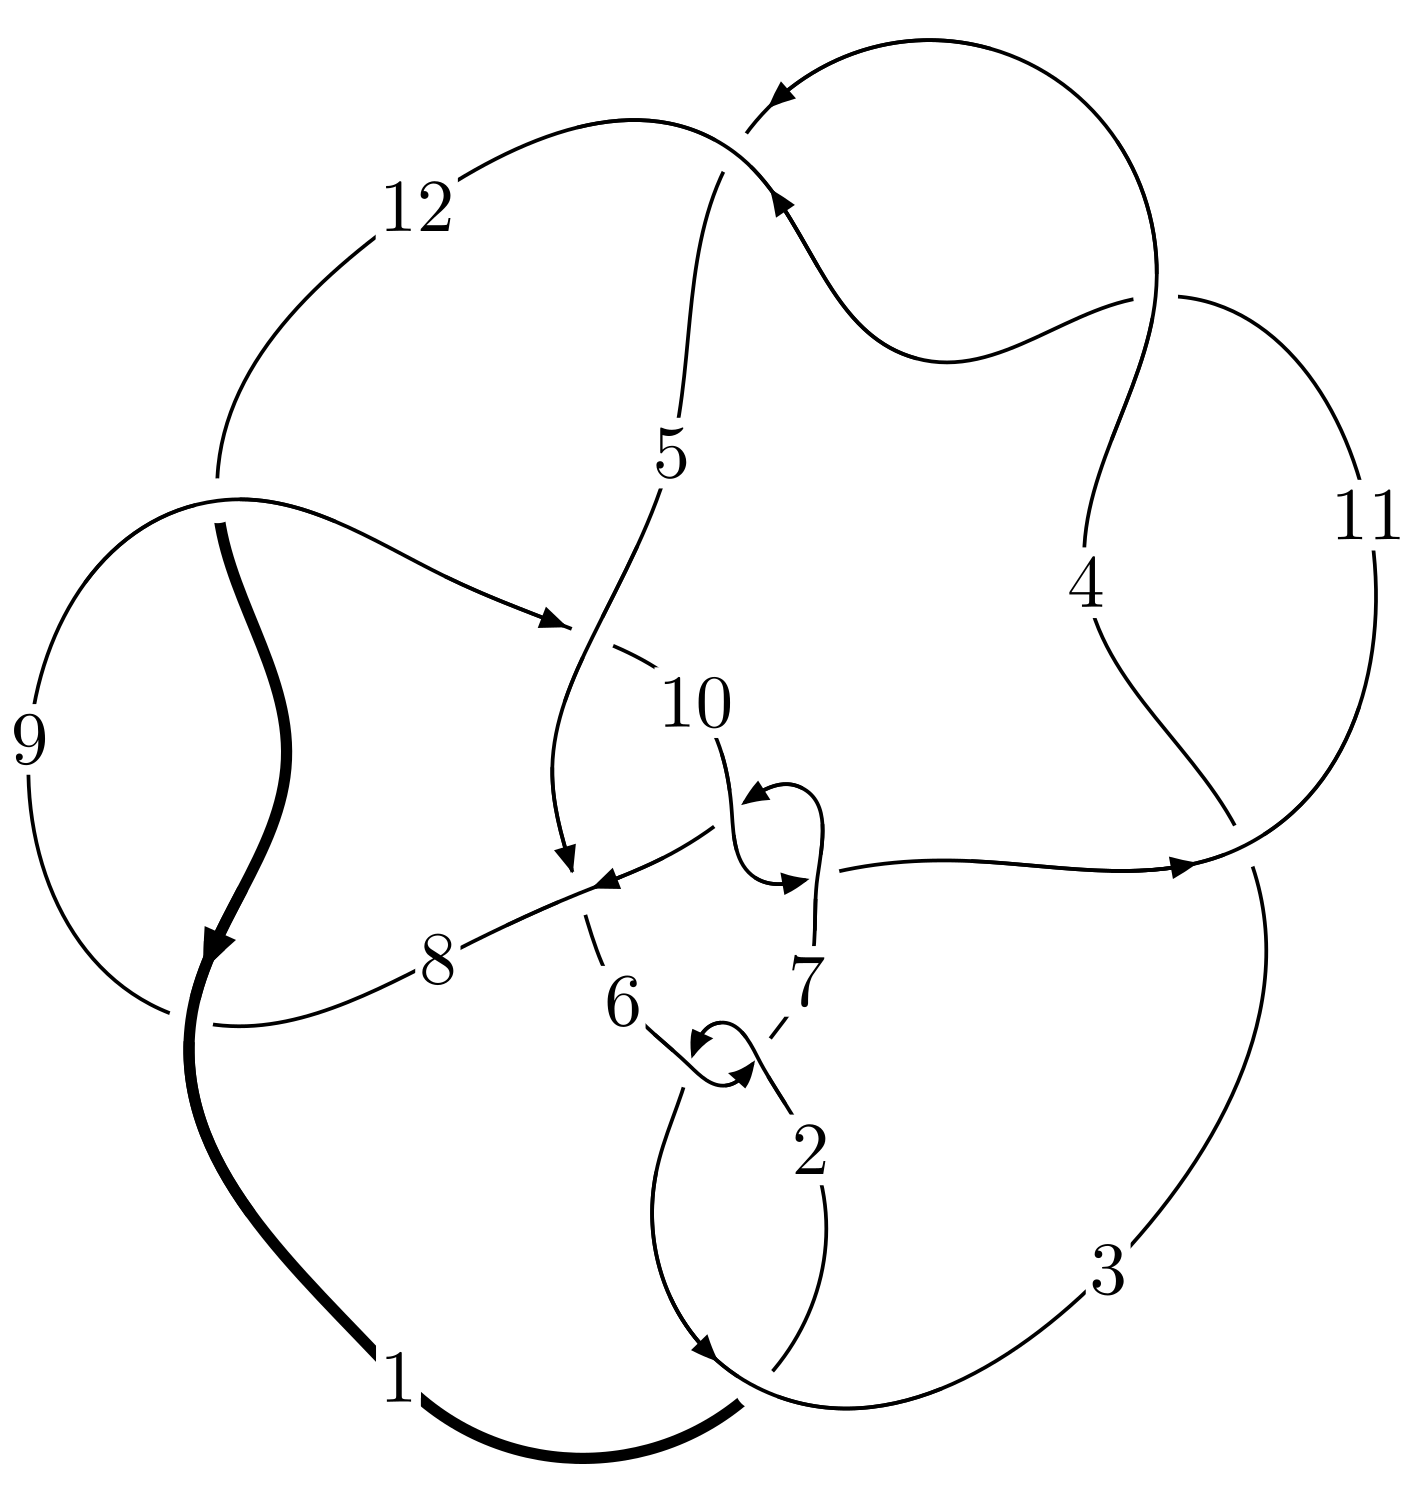
\includegraphics[width=112pt]{../../../GIT/diagram.site/Diagrams/png/1289_12a_0488.png}\\
\ \ \ A knot diagram\footnotemark}&
\allowdisplaybreaks
\textbf{Linearized knot diagam} \\
\cline{2-2}
 &
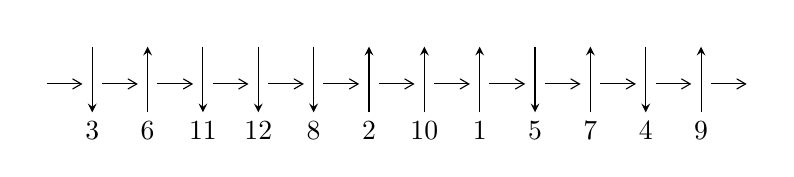
\begin{tikzpicture}[x=20pt, y=17pt]
	% nodes
	\node (C0) at (0, 0) {};
	\node (C1) at (1, 0) {};
	\node (C1U) at (1, +1) {};
	\node (C1D) at (1, -1) {3};

	\node (C2) at (2, 0) {};
	\node (C2U) at (2, +1) {};
	\node (C2D) at (2, -1) {6};

	\node (C3) at (3, 0) {};
	\node (C3U) at (3, +1) {};
	\node (C3D) at (3, -1) {11};

	\node (C4) at (4, 0) {};
	\node (C4U) at (4, +1) {};
	\node (C4D) at (4, -1) {12};

	\node (C5) at (5, 0) {};
	\node (C5U) at (5, +1) {};
	\node (C5D) at (5, -1) {8};

	\node (C6) at (6, 0) {};
	\node (C6U) at (6, +1) {};
	\node (C6D) at (6, -1) {2};

	\node (C7) at (7, 0) {};
	\node (C7U) at (7, +1) {};
	\node (C7D) at (7, -1) {10};

	\node (C8) at (8, 0) {};
	\node (C8U) at (8, +1) {};
	\node (C8D) at (8, -1) {1};

	\node (C9) at (9, 0) {};
	\node (C9U) at (9, +1) {};
	\node (C9D) at (9, -1) {5};

	\node (C10) at (10, 0) {};
	\node (C10U) at (10, +1) {};
	\node (C10D) at (10, -1) {7};

	\node (C11) at (11, 0) {};
	\node (C11U) at (11, +1) {};
	\node (C11D) at (11, -1) {4};

	\node (C12) at (12, 0) {};
	\node (C12U) at (12, +1) {};
	\node (C12D) at (12, -1) {9};
	\node (C13) at (13, 0) {};

	% arrows
	\draw[->,>={angle 60}]
	(C0) edge (C1) (C1) edge (C2) (C2) edge (C3) (C3) edge (C4) (C4) edge (C5) (C5) edge (C6) (C6) edge (C7) (C7) edge (C8) (C8) edge (C9) (C9) edge (C10) (C10) edge (C11) (C11) edge (C12) (C12) edge (C13) ;	\draw[->,>=stealth]
	(C1U) edge (C1D) (C2D) edge (C2U) (C3U) edge (C3D) (C4U) edge (C4D) (C5U) edge (C5D) (C6D) edge (C6U) (C7D) edge (C7U) (C8D) edge (C8U) (C9U) edge (C9D) (C10D) edge (C10U) (C11U) edge (C11D) (C12D) edge (C12U) ;
	\end{tikzpicture} \\
\hhline{~~} \\& 
\textbf{Solving Sequence} \\ \cline{2-2} 
 &
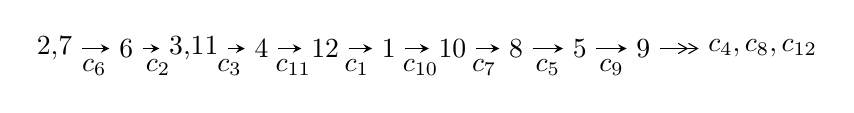
\begin{tikzpicture}[x=23pt, y=7pt]
	% node
	\node (A0) at (-1/8, 0) {2,7};
	\node (A1) at (1, 0) {6};
	\node (A2) at (33/16, 0) {3,11};
	\node (A3) at (25/8, 0) {4};
	\node (A4) at (33/8, 0) {12};
	\node (A5) at (41/8, 0) {1};
	\node (A6) at (49/8, 0) {10};
	\node (A7) at (57/8, 0) {8};
	\node (A8) at (65/8, 0) {5};
	\node (A9) at (73/8, 0) {9};
	\node (C1) at (1/2, -1) {$c_{6}$};
	\node (C2) at (3/2, -1) {$c_{2}$};
	\node (C3) at (21/8, -1) {$c_{3}$};
	\node (C4) at (29/8, -1) {$c_{11}$};
	\node (C5) at (37/8, -1) {$c_{1}$};
	\node (C6) at (45/8, -1) {$c_{10}$};
	\node (C7) at (53/8, -1) {$c_{7}$};
	\node (C8) at (61/8, -1) {$c_{5}$};
	\node (C9) at (69/8, -1) {$c_{9}$};
	\node (A10) at (11, 0) {$c_{4},c_{8},c_{12}$};

	% edge
	\draw[->,>=stealth]	
	(A0) edge (A1) (A1) edge (A2) (A2) edge (A3) (A3) edge (A4) (A4) edge (A5) (A5) edge (A6) (A6) edge (A7) (A7) edge (A8) (A8) edge (A9) ;
	\draw[->>,>={angle 60}]	
	(A9) edge (A10);
\end{tikzpicture} \\ 

\end{tabular} \\

\footnotetext{
The image of knot diagram is generated by the software ``\textbf{Draw programme}" developed by Andrew Bartholomew(\url{http://www.layer8.co.uk/maths/draw/index.htm\#Running-draw}), where we modified some parts for our purpose(\url{https://github.com/CATsTAILs/LinksPainter}).
}\phantom \\ \newline 
\centering \textbf{Ideals for irreducible components\footnotemark of $X_{\text{par}}$} 
 
\begin{align*}
I^u_{1}&=\langle 
-1.65087\times10^{248} u^{118}+2.72906\times10^{248} u^{117}+\cdots+2.57855\times10^{249} b+1.16888\times10^{250},\\
\phantom{I^u_{1}}&\phantom{= \langle  }1.43063\times10^{250} u^{118}-6.87154\times10^{249} u^{117}+\cdots+4.89925\times10^{250} a-3.41245\times10^{250},\\
\phantom{I^u_{1}}&\phantom{= \langle  }u^{119}+30 u^{117}+\cdots-45 u+19\rangle \\
I^u_{2}&=\langle 
13267248 u^{31}+55919199 u^{30}+\cdots+2842907 b+19270283,\\
\phantom{I^u_{2}}&\phantom{= \langle  }9664909 u^{31}+35225564 u^{30}+\cdots+2842907 a+34133711,\;u^{32}+3 u^{31}+\cdots+u+1\rangle \\
\\
\end{align*}
\raggedright * 2 irreducible components of $\dim_{\mathbb{C}}=0$, with total 151 representations.\\
\footnotetext{All coefficients of polynomials are rational numbers. But the coefficients are sometimes approximated in decimal forms when there is not enough margin.}
\newpage
\renewcommand{\arraystretch}{1}
\centering \section*{I. $I^u_{1}= \langle -1.65\times10^{248} u^{118}+2.73\times10^{248} u^{117}+\cdots+2.58\times10^{249} b+1.17\times10^{250},\;1.43\times10^{250} u^{118}-6.87\times10^{249} u^{117}+\cdots+4.90\times10^{250} a-3.41\times10^{250},\;u^{119}+30 u^{117}+\cdots-45 u+19 \rangle$}
\flushleft \textbf{(i) Arc colorings}\\
\begin{tabular}{m{7pt} m{180pt} m{7pt} m{180pt} }
\flushright $a_{2}=$&$\begin{pmatrix}0\\u\end{pmatrix}$ \\
\flushright $a_{7}=$&$\begin{pmatrix}1\\0\end{pmatrix}$ \\
\flushright $a_{6}=$&$\begin{pmatrix}1\\u^2\end{pmatrix}$ \\
\flushright $a_{3}=$&$\begin{pmatrix}u\\u^3+u\end{pmatrix}$ \\
\flushright $a_{11}=$&$\begin{pmatrix}-0.292010 u^{118}+0.140257 u^{117}+\cdots-3.40277 u+0.696526\\0.0640231 u^{118}-0.105837 u^{117}+\cdots+5.52131 u-4.53310\end{pmatrix}$ \\
\flushright $a_{4}=$&$\begin{pmatrix}0.762522 u^{118}+0.270935 u^{117}+\cdots+39.1067 u-1.83376\\-0.352113 u^{118}+0.127974 u^{117}+\cdots-14.0857 u+0.578793\end{pmatrix}$ \\
\flushright $a_{12}=$&$\begin{pmatrix}-0.245358 u^{118}-0.0980200 u^{117}+\cdots-29.2465 u+7.46517\\-0.667052 u^{118}-0.0422577 u^{117}+\cdots-19.9808 u+0.289591\end{pmatrix}$ \\
\flushright $a_{1}=$&$\begin{pmatrix}u^3\\u^5+u^3+u\end{pmatrix}$ \\
\flushright $a_{10}=$&$\begin{pmatrix}-0.356033 u^{118}+0.246094 u^{117}+\cdots-8.92408 u+5.22962\\0.0640231 u^{118}-0.105837 u^{117}+\cdots+5.52131 u-4.53310\end{pmatrix}$ \\
\flushright $a_{8}=$&$\begin{pmatrix}-0.0171301 u^{118}-0.576448 u^{117}+\cdots+57.5877 u-21.0304\\0.146326 u^{118}+0.138789 u^{117}+\cdots-4.58356 u-0.367599\end{pmatrix}$ \\
\flushright $a_{5}=$&$\begin{pmatrix}-0.233262 u^{118}+0.761502 u^{117}+\cdots-46.6619 u+20.3764\\0.272002 u^{118}+0.183648 u^{117}+\cdots-4.44302 u+5.56541\end{pmatrix}$ \\
\flushright $a_{9}=$&$\begin{pmatrix}-0.0232125 u^{118}-0.478908 u^{117}+\cdots+49.3275 u-17.7018\\0.171123 u^{118}+0.0186106 u^{117}+\cdots+8.48928 u-4.65434\end{pmatrix}$\\&\end{tabular}
\flushleft \textbf{(ii) Obstruction class $= -1$}\\~\\
\flushleft \textbf{(iii) Cusp Shapes $= 1.15974 u^{118}+0.0943856 u^{117}+\cdots+31.1713 u+1.75865$}\\~\\
\newpage\renewcommand{\arraystretch}{1}
\flushleft \textbf{(iv) u-Polynomials at the component}\newline \\
\begin{tabular}{m{50pt}|m{274pt}}
Crossings & \hspace{64pt}u-Polynomials at each crossing \\
\hline $$\begin{aligned}c_{1}\end{aligned}$$&$\begin{aligned}
&u^{119}+60 u^{118}+\cdots-4929 u-361
\end{aligned}$\\
\hline $$\begin{aligned}c_{2},c_{6}\end{aligned}$$&$\begin{aligned}
&u^{119}+30 u^{117}+\cdots-45 u+19
\end{aligned}$\\
\hline $$\begin{aligned}c_{3},c_{4},c_{11}\end{aligned}$$&$\begin{aligned}
&u^{119}+3 u^{118}+\cdots-236 u+29
\end{aligned}$\\
\hline $$\begin{aligned}c_{5}\end{aligned}$$&$\begin{aligned}
&u^{119}-8 u^{118}+\cdots+84246 u-6676
\end{aligned}$\\
\hline $$\begin{aligned}c_{7},c_{10}\end{aligned}$$&$\begin{aligned}
&u^{119}+6 u^{118}+\cdots-1800 u-200
\end{aligned}$\\
\hline $$\begin{aligned}c_{8},c_{12}\end{aligned}$$&$\begin{aligned}
&u^{119}-3 u^{118}+\cdots-1224 u+2727
\end{aligned}$\\
\hline $$\begin{aligned}c_{9}\end{aligned}$$&$\begin{aligned}
&u^{119}+2 u^{118}+\cdots-715329093 u-124700713
\end{aligned}$\\
\hline
\end{tabular}\\~\\
\newpage\renewcommand{\arraystretch}{1}
\flushleft \textbf{(v) Riley Polynomials at the component}\newline \\
\begin{tabular}{m{50pt}|m{274pt}}
Crossings & \hspace{64pt}Riley Polynomials at each crossing \\
\hline $$\begin{aligned}c_{1}\end{aligned}$$&$\begin{aligned}
&y^{119}+12 y^{118}+\cdots+9244951 y-130321
\end{aligned}$\\
\hline $$\begin{aligned}c_{2},c_{6}\end{aligned}$$&$\begin{aligned}
&y^{119}+60 y^{118}+\cdots-4929 y-361
\end{aligned}$\\
\hline $$\begin{aligned}c_{3},c_{4},c_{11}\end{aligned}$$&$\begin{aligned}
&y^{119}-131 y^{118}+\cdots-91218 y-841
\end{aligned}$\\
\hline $$\begin{aligned}c_{5}\end{aligned}$$&$\begin{aligned}
&y^{119}-30 y^{118}+\cdots+2009862604 y-44568976
\end{aligned}$\\
\hline $$\begin{aligned}c_{7},c_{10}\end{aligned}$$&$\begin{aligned}
&y^{119}+84 y^{118}+\cdots-1890400 y-40000
\end{aligned}$\\
\hline $$\begin{aligned}c_{8},c_{12}\end{aligned}$$&$\begin{aligned}
&y^{119}+89 y^{118}+\cdots-366139602 y-7436529
\end{aligned}$\\
\hline $$\begin{aligned}c_{9}\end{aligned}$$&$\begin{aligned}
&y^{119}-62 y^{118}+\cdots+559579641828065865 y-15550267822708369
\end{aligned}$\\
\hline
\end{tabular}\\~\\
\newpage\flushleft \textbf{(vi) Complex Volumes and Cusp Shapes}
$$\begin{array}{c|c|c}  
\text{Solutions to }I^u_{1}& \I (\text{vol} + \sqrt{-1}CS) & \text{Cusp shape}\\
 \hline 
\begin{aligned}
u &= -0.078496 + 1.006620 I \\
a &= -0.066856 + 0.754688 I \\
b &= \phantom{-}0.594329 + 0.314337 I\end{aligned}
 & -5.14761 + 1.62016 I & \phantom{-0.000000 } 0 \\ \hline\begin{aligned}
u &= -0.078496 - 1.006620 I \\
a &= -0.066856 - 0.754688 I \\
b &= \phantom{-}0.594329 - 0.314337 I\end{aligned}
 & -5.14761 - 1.62016 I & \phantom{-0.000000 } 0 \\ \hline\begin{aligned}
u &= \phantom{-}0.915404 + 0.371979 I \\
a &= -0.64387 + 1.32526 I \\
b &= -0.52974 + 1.37782 I\end{aligned}
 & -6.73097 - 5.70611 I & \phantom{-0.000000 } 0 \\ \hline\begin{aligned}
u &= \phantom{-}0.915404 - 0.371979 I \\
a &= -0.64387 - 1.32526 I \\
b &= -0.52974 - 1.37782 I\end{aligned}
 & -6.73097 + 5.70611 I & \phantom{-0.000000 } 0 \\ \hline\begin{aligned}
u &= -0.971804 + 0.146641 I \\
a &= -1.073250 + 0.068787 I \\
b &= -0.607735 + 0.718070 I\end{aligned}
 & -4.79116 - 2.35384 I & \phantom{-0.000000 } 0 \\ \hline\begin{aligned}
u &= -0.971804 - 0.146641 I \\
a &= -1.073250 - 0.068787 I \\
b &= -0.607735 - 0.718070 I\end{aligned}
 & -4.79116 + 2.35384 I & \phantom{-0.000000 } 0 \\ \hline\begin{aligned}
u &= \phantom{-}0.610950 + 0.757773 I \\
a &= \phantom{-}0.088819 + 1.042710 I \\
b &= -0.365398 + 0.311650 I\end{aligned}
 & \phantom{-}0.348231 + 0.671437 I & \phantom{-0.000000 } 0 \\ \hline\begin{aligned}
u &= \phantom{-}0.610950 - 0.757773 I \\
a &= \phantom{-}0.088819 - 1.042710 I \\
b &= -0.365398 - 0.311650 I\end{aligned}
 & \phantom{-}0.348231 - 0.671437 I & \phantom{-0.000000 } 0 \\ \hline\begin{aligned}
u &= -0.959729 + 0.055167 I \\
a &= \phantom{-}0.740938 - 0.325683 I \\
b &= \phantom{-}0.188991 - 0.919450 I\end{aligned}
 & -3.27901 - 1.00446 I & \phantom{-0.000000 } 0 \\ \hline\begin{aligned}
u &= -0.959729 - 0.055167 I \\
a &= \phantom{-}0.740938 + 0.325683 I \\
b &= \phantom{-}0.188991 + 0.919450 I\end{aligned}
 & -3.27901 + 1.00446 I & \phantom{-0.000000 } 0\\
 \hline 
 \end{array}$$\newpage$$\begin{array}{c|c|c}  
\text{Solutions to }I^u_{1}& \I (\text{vol} + \sqrt{-1}CS) & \text{Cusp shape}\\
 \hline 
\begin{aligned}
u &= -0.483520 + 0.920992 I \\
a &= -0.761211 - 1.077530 I \\
b &= -1.178340 - 0.167584 I\end{aligned}
 & \phantom{-}1.52635 - 2.31331 I & \phantom{-0.000000 } 0 \\ \hline\begin{aligned}
u &= -0.483520 - 0.920992 I \\
a &= -0.761211 + 1.077530 I \\
b &= -1.178340 + 0.167584 I\end{aligned}
 & \phantom{-}1.52635 + 2.31331 I & \phantom{-0.000000 } 0 \\ \hline\begin{aligned}
u &= \phantom{-}0.557621 + 0.879341 I \\
a &= -1.156820 - 0.285053 I \\
b &= -0.682531 - 0.473571 I\end{aligned}
 & -0.04577 + 3.96034 I & \phantom{-0.000000 } 0 \\ \hline\begin{aligned}
u &= \phantom{-}0.557621 - 0.879341 I \\
a &= -1.156820 + 0.285053 I \\
b &= -0.682531 + 0.473571 I\end{aligned}
 & -0.04577 - 3.96034 I & \phantom{-0.000000 } 0 \\ \hline\begin{aligned}
u &= \phantom{-}1.022200 + 0.281034 I \\
a &= \phantom{-}0.758036 - 0.978664 I \\
b &= \phantom{-}0.53987 - 1.35453 I\end{aligned}
 & -11.3125 - 11.9691 I & \phantom{-0.000000 } 0 \\ \hline\begin{aligned}
u &= \phantom{-}1.022200 - 0.281034 I \\
a &= \phantom{-}0.758036 + 0.978664 I \\
b &= \phantom{-}0.53987 + 1.35453 I\end{aligned}
 & -11.3125 + 11.9691 I & \phantom{-0.000000 } 0 \\ \hline\begin{aligned}
u &= \phantom{-}0.001806 + 0.927592 I \\
a &= \phantom{-}0.78130 - 2.73177 I \\
b &= \phantom{-}0.345980 + 0.917689 I\end{aligned}
 & -9.46778 + 4.21449 I & \phantom{-0.000000 } 0 \\ \hline\begin{aligned}
u &= \phantom{-}0.001806 - 0.927592 I \\
a &= \phantom{-}0.78130 + 2.73177 I \\
b &= \phantom{-}0.345980 - 0.917689 I\end{aligned}
 & -9.46778 - 4.21449 I & \phantom{-0.000000 } 0 \\ \hline\begin{aligned}
u &= -0.297606 + 1.031700 I \\
a &= \phantom{-}0.945429 + 0.802633 I \\
b &= -0.094023 - 1.195090 I\end{aligned}
 & -4.19251 + 1.14824 I & \phantom{-0.000000 } 0 \\ \hline\begin{aligned}
u &= -0.297606 - 1.031700 I \\
a &= \phantom{-}0.945429 - 0.802633 I \\
b &= -0.094023 + 1.195090 I\end{aligned}
 & -4.19251 - 1.14824 I & \phantom{-0.000000 } 0\\
 \hline 
 \end{array}$$\newpage$$\begin{array}{c|c|c}  
\text{Solutions to }I^u_{1}& \I (\text{vol} + \sqrt{-1}CS) & \text{Cusp shape}\\
 \hline 
\begin{aligned}
u &= -0.690673 + 0.825474 I \\
a &= \phantom{-}0.150303 - 0.265933 I \\
b &= \phantom{-}0.425489 + 0.705888 I\end{aligned}
 & -5.15633 - 4.20772 I & \phantom{-0.000000 } 0 \\ \hline\begin{aligned}
u &= -0.690673 - 0.825474 I \\
a &= \phantom{-}0.150303 + 0.265933 I \\
b &= \phantom{-}0.425489 - 0.705888 I\end{aligned}
 & -5.15633 + 4.20772 I & \phantom{-0.000000 } 0 \\ \hline\begin{aligned}
u &= -0.861339 + 0.322459 I \\
a &= \phantom{-}0.654805 + 0.598022 I \\
b &= \phantom{-}0.445085 + 1.258140 I\end{aligned}
 & -4.09112 + 7.73397 I & \phantom{-0.000000 } 0 \\ \hline\begin{aligned}
u &= -0.861339 - 0.322459 I \\
a &= \phantom{-}0.654805 - 0.598022 I \\
b &= \phantom{-}0.445085 - 1.258140 I\end{aligned}
 & -4.09112 - 7.73397 I & \phantom{-0.000000 } 0 \\ \hline\begin{aligned}
u &= \phantom{-}0.755924 + 0.473545 I \\
a &= -0.289346 - 0.331743 I \\
b &= -0.254049 - 0.757979 I\end{aligned}
 & \phantom{-}0.21533 + 1.51725 I & \phantom{-0.000000 } 0 \\ \hline\begin{aligned}
u &= \phantom{-}0.755924 - 0.473545 I \\
a &= -0.289346 + 0.331743 I \\
b &= -0.254049 + 0.757979 I\end{aligned}
 & \phantom{-}0.21533 - 1.51725 I & \phantom{-0.000000 } 0 \\ \hline\begin{aligned}
u &= -0.247532 + 1.081640 I \\
a &= -1.69931 - 0.65268 I \\
b &= -0.211828 - 0.379548 I\end{aligned}
 & -10.56410 - 5.20427 I & \phantom{-0.000000 } 0 \\ \hline\begin{aligned}
u &= -0.247532 - 1.081640 I \\
a &= -1.69931 + 0.65268 I \\
b &= -0.211828 + 0.379548 I\end{aligned}
 & -10.56410 + 5.20427 I & \phantom{-0.000000 } 0 \\ \hline\begin{aligned}
u &= \phantom{-}0.391633 + 1.039930 I \\
a &= -1.14573 + 1.23527 I \\
b &= -0.344583 - 1.276950 I\end{aligned}
 & -3.11586 + 3.83174 I & \phantom{-0.000000 } 0 \\ \hline\begin{aligned}
u &= \phantom{-}0.391633 - 1.039930 I \\
a &= -1.14573 - 1.23527 I \\
b &= -0.344583 + 1.276950 I\end{aligned}
 & -3.11586 - 3.83174 I & \phantom{-0.000000 } 0\\
 \hline 
 \end{array}$$\newpage$$\begin{array}{c|c|c}  
\text{Solutions to }I^u_{1}& \I (\text{vol} + \sqrt{-1}CS) & \text{Cusp shape}\\
 \hline 
\begin{aligned}
u &= -0.346137 + 1.071550 I \\
a &= \phantom{-}0.095834 + 0.830795 I \\
b &= -0.11817 - 1.56259 I\end{aligned}
 & -14.9180 + 0.0272 I & \phantom{-0.000000 } 0 \\ \hline\begin{aligned}
u &= -0.346137 - 1.071550 I \\
a &= \phantom{-}0.095834 - 0.830795 I \\
b &= -0.11817 + 1.56259 I\end{aligned}
 & -14.9180 - 0.0272 I & \phantom{-0.000000 } 0 \\ \hline\begin{aligned}
u &= \phantom{-}0.624726 + 0.597146 I \\
a &= \phantom{-}0.588397 + 0.077030 I \\
b &= \phantom{-}0.382126 - 0.228734 I\end{aligned}
 & -0.091081 + 1.070900 I & \phantom{-0.000000 } 0 \\ \hline\begin{aligned}
u &= \phantom{-}0.624726 - 0.597146 I \\
a &= \phantom{-}0.588397 - 0.077030 I \\
b &= \phantom{-}0.382126 + 0.228734 I\end{aligned}
 & -0.091081 - 1.070900 I & \phantom{-0.000000 } 0 \\ \hline\begin{aligned}
u &= -0.480364 + 0.710793 I \\
a &= -1.43891 - 0.64056 I \\
b &= -0.977189 + 0.403194 I\end{aligned}
 & \phantom{-}2.15917 - 1.67533 I & \phantom{-0.000000 } 0 \\ \hline\begin{aligned}
u &= -0.480364 - 0.710793 I \\
a &= -1.43891 + 0.64056 I \\
b &= -0.977189 - 0.403194 I\end{aligned}
 & \phantom{-}2.15917 + 1.67533 I & \phantom{-0.000000 } 0 \\ \hline\begin{aligned}
u &= \phantom{-}0.397106 + 1.070930 I \\
a &= -2.06076 + 1.01698 I \\
b &= -0.018775 - 1.148820 I\end{aligned}
 & -7.02483 + 1.08003 I & \phantom{-0.000000 } 0 \\ \hline\begin{aligned}
u &= \phantom{-}0.397106 - 1.070930 I \\
a &= -2.06076 - 1.01698 I \\
b &= -0.018775 + 1.148820 I\end{aligned}
 & -7.02483 - 1.08003 I & \phantom{-0.000000 } 0 \\ \hline\begin{aligned}
u &= -0.449317 + 1.052270 I \\
a &= \phantom{-}0.803311 + 0.104774 I \\
b &= \phantom{-}0.510546 + 0.420152 I\end{aligned}
 & -5.15832 - 3.39168 I & \phantom{-0.000000 } 0 \\ \hline\begin{aligned}
u &= -0.449317 - 1.052270 I \\
a &= \phantom{-}0.803311 - 0.104774 I \\
b &= \phantom{-}0.510546 - 0.420152 I\end{aligned}
 & -5.15832 + 3.39168 I & \phantom{-0.000000 } 0\\
 \hline 
 \end{array}$$\newpage$$\begin{array}{c|c|c}  
\text{Solutions to }I^u_{1}& \I (\text{vol} + \sqrt{-1}CS) & \text{Cusp shape}\\
 \hline 
\begin{aligned}
u &= \phantom{-}0.340211 + 1.097430 I \\
a &= -0.483940 - 0.075688 I \\
b &= \phantom{-}0.52633 - 1.74736 I\end{aligned}
 & -15.3194 + 3.5604 I & \phantom{-0.000000 } 0 \\ \hline\begin{aligned}
u &= \phantom{-}0.340211 - 1.097430 I \\
a &= -0.483940 + 0.075688 I \\
b &= \phantom{-}0.52633 + 1.74736 I\end{aligned}
 & -15.3194 - 3.5604 I & \phantom{-0.000000 } 0 \\ \hline\begin{aligned}
u &= -0.376858 + 1.086750 I \\
a &= \phantom{-}1.80905 + 0.75040 I \\
b &= \phantom{-}0.622858 - 1.182940 I\end{aligned}
 & -7.24480 - 3.53534 I & \phantom{-0.000000 } 0 \\ \hline\begin{aligned}
u &= -0.376858 - 1.086750 I \\
a &= \phantom{-}1.80905 - 0.75040 I \\
b &= \phantom{-}0.622858 + 1.182940 I\end{aligned}
 & -7.24480 + 3.53534 I & \phantom{-0.000000 } 0 \\ \hline\begin{aligned}
u &= -0.694027 + 0.468933 I \\
a &= \phantom{-}1.232930 + 0.362811 I \\
b &= \phantom{-}0.833219 - 0.067656 I\end{aligned}
 & -0.41000 + 3.05649 I & \phantom{-0.000000 } 0. - 3.81841 I \\ \hline\begin{aligned}
u &= -0.694027 - 0.468933 I \\
a &= \phantom{-}1.232930 - 0.362811 I \\
b &= \phantom{-}0.833219 + 0.067656 I\end{aligned}
 & -0.41000 - 3.05649 I & \phantom{-0.000000 -}0. + 3.81841 I \\ \hline\begin{aligned}
u &= \phantom{-}0.320264 + 1.120320 I \\
a &= \phantom{-}0.795246 - 1.083370 I \\
b &= \phantom{-}1.078340 - 0.475511 I\end{aligned}
 & -11.25190 - 3.18862 I & \phantom{-0.000000 } 0 \\ \hline\begin{aligned}
u &= \phantom{-}0.320264 - 1.120320 I \\
a &= \phantom{-}0.795246 + 1.083370 I \\
b &= \phantom{-}1.078340 + 0.475511 I\end{aligned}
 & -11.25190 + 3.18862 I & \phantom{-0.000000 } 0 \\ \hline\begin{aligned}
u &= \phantom{-}0.456472 + 1.081110 I \\
a &= -0.96919 + 1.09392 I \\
b &= -1.55906 + 0.30538 I\end{aligned}
 & -4.93294 + 3.53621 I & \phantom{-0.000000 } 0 \\ \hline\begin{aligned}
u &= \phantom{-}0.456472 - 1.081110 I \\
a &= -0.96919 - 1.09392 I \\
b &= -1.55906 - 0.30538 I\end{aligned}
 & -4.93294 - 3.53621 I & \phantom{-0.000000 } 0\\
 \hline 
 \end{array}$$\newpage$$\begin{array}{c|c|c}  
\text{Solutions to }I^u_{1}& \I (\text{vol} + \sqrt{-1}CS) & \text{Cusp shape}\\
 \hline 
\begin{aligned}
u &= -0.048098 + 0.813192 I \\
a &= \phantom{-}0.546020 - 1.277930 I \\
b &= \phantom{-}0.10854 + 1.69149 I\end{aligned}
 & -13.22850 - 1.96623 I & -4.87577 + 2.86715 I \\ \hline\begin{aligned}
u &= -0.048098 - 0.813192 I \\
a &= \phantom{-}0.546020 + 1.277930 I \\
b &= \phantom{-}0.10854 - 1.69149 I\end{aligned}
 & -13.22850 + 1.96623 I & -4.87577 - 2.86715 I \\ \hline\begin{aligned}
u &= \phantom{-}0.783036 + 0.906435 I \\
a &= \phantom{-}0.732493 - 0.007307 I \\
b &= \phantom{-}0.282695 + 0.746721 I\end{aligned}
 & -1.02424 + 4.22944 I & \phantom{-0.000000 } 0 \\ \hline\begin{aligned}
u &= \phantom{-}0.783036 - 0.906435 I \\
a &= \phantom{-}0.732493 + 0.007307 I \\
b &= \phantom{-}0.282695 - 0.746721 I\end{aligned}
 & -1.02424 - 4.22944 I & \phantom{-0.000000 } 0 \\ \hline\begin{aligned}
u &= -0.590224 + 1.044060 I \\
a &= \phantom{-}0.791102 + 0.738149 I \\
b &= \phantom{-}0.953043 - 0.051008 I\end{aligned}
 & -2.07376 - 7.99377 I & \phantom{-0.000000 } 0 \\ \hline\begin{aligned}
u &= -0.590224 - 1.044060 I \\
a &= \phantom{-}0.791102 - 0.738149 I \\
b &= \phantom{-}0.953043 + 0.051008 I\end{aligned}
 & -2.07376 + 7.99377 I & \phantom{-0.000000 } 0 \\ \hline\begin{aligned}
u &= \phantom{-}0.515096 + 1.085300 I \\
a &= \phantom{-}1.37662 - 0.49500 I \\
b &= \phantom{-}0.176990 + 1.072700 I\end{aligned}
 & -2.11670 + 3.02849 I & \phantom{-0.000000 } 0 \\ \hline\begin{aligned}
u &= \phantom{-}0.515096 - 1.085300 I \\
a &= \phantom{-}1.37662 + 0.49500 I \\
b &= \phantom{-}0.176990 - 1.072700 I\end{aligned}
 & -2.11670 - 3.02849 I & \phantom{-0.000000 } 0 \\ \hline\begin{aligned}
u &= \phantom{-}0.661505 + 1.003050 I \\
a &= \phantom{-}0.250669 - 0.344058 I \\
b &= \phantom{-}0.088473 + 0.250492 I\end{aligned}
 & -1.11997 + 4.05223 I & \phantom{-0.000000 } 0 \\ \hline\begin{aligned}
u &= \phantom{-}0.661505 - 1.003050 I \\
a &= \phantom{-}0.250669 + 0.344058 I \\
b &= \phantom{-}0.088473 - 0.250492 I\end{aligned}
 & -1.11997 - 4.05223 I & \phantom{-0.000000 } 0\\
 \hline 
 \end{array}$$\newpage$$\begin{array}{c|c|c}  
\text{Solutions to }I^u_{1}& \I (\text{vol} + \sqrt{-1}CS) & \text{Cusp shape}\\
 \hline 
\begin{aligned}
u &= -0.992539 + 0.678641 I \\
a &= -0.207770 + 0.955665 I \\
b &= -0.046228 + 1.099290 I\end{aligned}
 & -4.92580 - 0.78909 I & \phantom{-0.000000 } 0 \\ \hline\begin{aligned}
u &= -0.992539 - 0.678641 I \\
a &= -0.207770 - 0.955665 I \\
b &= -0.046228 - 1.099290 I\end{aligned}
 & -4.92580 + 0.78909 I & \phantom{-0.000000 } 0 \\ \hline\begin{aligned}
u &= \phantom{-}0.502054 + 1.093030 I \\
a &= \phantom{-}1.22292 - 1.16724 I \\
b &= \phantom{-}0.214525 + 1.380870 I\end{aligned}
 & -6.25245 + 6.03157 I & \phantom{-0.000000 } 0 \\ \hline\begin{aligned}
u &= \phantom{-}0.502054 - 1.093030 I \\
a &= \phantom{-}1.22292 + 1.16724 I \\
b &= \phantom{-}0.214525 - 1.380870 I\end{aligned}
 & -6.25245 - 6.03157 I & \phantom{-0.000000 } 0 \\ \hline\begin{aligned}
u &= \phantom{-}0.733796 + 0.280195 I \\
a &= \phantom{-}1.83401 - 0.78059 I \\
b &= \phantom{-}1.084740 + 0.057816 I\end{aligned}
 & -7.20334 - 6.18714 I & -2.58267 + 3.56489 I \\ \hline\begin{aligned}
u &= \phantom{-}0.733796 - 0.280195 I \\
a &= \phantom{-}1.83401 + 0.78059 I \\
b &= \phantom{-}1.084740 - 0.057816 I\end{aligned}
 & -7.20334 + 6.18714 I & -2.58267 - 3.56489 I \\ \hline\begin{aligned}
u &= -0.154870 + 1.212180 I \\
a &= -0.281737 - 1.085590 I \\
b &= \phantom{-}0.257713 + 1.193340 I\end{aligned}
 & -9.35505 + 4.62458 I & \phantom{-0.000000 } 0 \\ \hline\begin{aligned}
u &= -0.154870 - 1.212180 I \\
a &= -0.281737 + 1.085590 I \\
b &= \phantom{-}0.257713 - 1.193340 I\end{aligned}
 & -9.35505 - 4.62458 I & \phantom{-0.000000 } 0 \\ \hline\begin{aligned}
u &= \phantom{-}0.271992 + 0.726580 I \\
a &= -0.928303 + 0.091287 I \\
b &= -0.616444 + 1.054960 I\end{aligned}
 & -1.81332 - 0.95297 I & -7.18259 - 4.49578 I \\ \hline\begin{aligned}
u &= \phantom{-}0.271992 - 0.726580 I \\
a &= -0.928303 - 0.091287 I \\
b &= -0.616444 - 1.054960 I\end{aligned}
 & -1.81332 + 0.95297 I & -7.18259 + 4.49578 I\\
 \hline 
 \end{array}$$\newpage$$\begin{array}{c|c|c}  
\text{Solutions to }I^u_{1}& \I (\text{vol} + \sqrt{-1}CS) & \text{Cusp shape}\\
 \hline 
\begin{aligned}
u &= -0.543939 + 1.101550 I \\
a &= -1.65517 - 0.58118 I \\
b &= -0.52640 + 1.34651 I\end{aligned}
 & -2.49241 - 8.21984 I & \phantom{-0.000000 } 0 \\ \hline\begin{aligned}
u &= -0.543939 - 1.101550 I \\
a &= -1.65517 + 0.58118 I \\
b &= -0.52640 - 1.34651 I\end{aligned}
 & -2.49241 + 8.21984 I & \phantom{-0.000000 } 0 \\ \hline\begin{aligned}
u &= \phantom{-}0.067829 + 0.768409 I \\
a &= -0.96334 + 1.71841 I \\
b &= \phantom{-}0.266423 + 0.709161 I\end{aligned}
 & -5.13022 + 1.42643 I & -5.68961 - 4.05615 I \\ \hline\begin{aligned}
u &= \phantom{-}0.067829 - 0.768409 I \\
a &= -0.96334 - 1.71841 I \\
b &= \phantom{-}0.266423 - 0.709161 I\end{aligned}
 & -5.13022 - 1.42643 I & -5.68961 + 4.05615 I \\ \hline\begin{aligned}
u &= -0.547528 + 1.099960 I \\
a &= -2.12152 + 0.21831 I \\
b &= -0.210386 + 1.214010 I\end{aligned}
 & -13.4502 - 7.1902 I & \phantom{-0.000000 } 0 \\ \hline\begin{aligned}
u &= -0.547528 - 1.099960 I \\
a &= -2.12152 - 0.21831 I \\
b &= -0.210386 - 1.214010 I\end{aligned}
 & -13.4502 + 7.1902 I & \phantom{-0.000000 } 0 \\ \hline\begin{aligned}
u &= -0.683513 + 0.356634 I \\
a &= -0.618553 - 0.865136 I \\
b &= -0.488959 - 1.144820 I\end{aligned}
 & -0.31858 + 3.47575 I & \phantom{-}1.97968 - 4.35878 I \\ \hline\begin{aligned}
u &= -0.683513 - 0.356634 I \\
a &= -0.618553 + 0.865136 I \\
b &= -0.488959 + 1.144820 I\end{aligned}
 & -0.31858 - 3.47575 I & \phantom{-}1.97968 + 4.35878 I \\ \hline\begin{aligned}
u &= -0.652062 + 0.393739 I \\
a &= -0.80892 - 1.88179 I \\
b &= \phantom{-}0.016975 - 1.229550 I\end{aligned}
 & -11.36620 + 2.46799 I & -7.23736 - 0.73082 I \\ \hline\begin{aligned}
u &= -0.652062 - 0.393739 I \\
a &= -0.80892 + 1.88179 I \\
b &= \phantom{-}0.016975 + 1.229550 I\end{aligned}
 & -11.36620 - 2.46799 I & -7.23736 + 0.73082 I\\
 \hline 
 \end{array}$$\newpage$$\begin{array}{c|c|c}  
\text{Solutions to }I^u_{1}& \I (\text{vol} + \sqrt{-1}CS) & \text{Cusp shape}\\
 \hline 
\begin{aligned}
u &= -0.510279 + 1.132000 I \\
a &= -0.585905 - 0.278024 I \\
b &= \phantom{-}0.128771 + 1.287050 I\end{aligned}
 & -6.19002 - 3.93927 I & \phantom{-0.000000 } 0 \\ \hline\begin{aligned}
u &= -0.510279 - 1.132000 I \\
a &= -0.585905 + 0.278024 I \\
b &= \phantom{-}0.128771 - 1.287050 I\end{aligned}
 & -6.19002 + 3.93927 I & \phantom{-0.000000 } 0 \\ \hline\begin{aligned}
u &= \phantom{-}0.543113 + 1.116850 I \\
a &= \phantom{-}2.05669 - 0.15147 I \\
b &= \phantom{-}0.79420 + 1.37241 I\end{aligned}
 & -13.8603 + 3.9134 I & \phantom{-0.000000 } 0 \\ \hline\begin{aligned}
u &= \phantom{-}0.543113 - 1.116850 I \\
a &= \phantom{-}2.05669 + 0.15147 I \\
b &= \phantom{-}0.79420 - 1.37241 I\end{aligned}
 & -13.8603 - 3.9134 I & \phantom{-0.000000 } 0 \\ \hline\begin{aligned}
u &= \phantom{-}0.674419 + 0.342927 I \\
a &= \phantom{-}1.00312 - 2.08896 I \\
b &= \phantom{-}0.53117 - 1.32772 I\end{aligned}
 & -11.59410 + 0.83287 I & -6.75862 - 0.75002 I \\ \hline\begin{aligned}
u &= \phantom{-}0.674419 - 0.342927 I \\
a &= \phantom{-}1.00312 + 2.08896 I \\
b &= \phantom{-}0.53117 + 1.32772 I\end{aligned}
 & -11.59410 - 0.83287 I & -6.75862 + 0.75002 I \\ \hline\begin{aligned}
u &= \phantom{-}0.096088 + 1.248340 I \\
a &= \phantom{-}0.285246 - 0.360833 I \\
b &= -0.21055 + 1.53910 I\end{aligned}
 & -12.56200 - 2.66586 I & \phantom{-0.000000 } 0 \\ \hline\begin{aligned}
u &= \phantom{-}0.096088 - 1.248340 I \\
a &= \phantom{-}0.285246 + 0.360833 I \\
b &= -0.21055 - 1.53910 I\end{aligned}
 & -12.56200 + 2.66586 I & \phantom{-0.000000 } 0 \\ \hline\begin{aligned}
u &= \phantom{-}0.538749 + 1.136970 I \\
a &= \phantom{-}0.972594 - 0.790349 I \\
b &= \phantom{-}1.369210 - 0.022434 I\end{aligned}
 & -9.7097 + 11.0092 I & \phantom{-0.000000 } 0 \\ \hline\begin{aligned}
u &= \phantom{-}0.538749 - 1.136970 I \\
a &= \phantom{-}0.972594 + 0.790349 I \\
b &= \phantom{-}1.369210 + 0.022434 I\end{aligned}
 & -9.7097 - 11.0092 I & \phantom{-0.000000 } 0\\
 \hline 
 \end{array}$$\newpage$$\begin{array}{c|c|c}  
\text{Solutions to }I^u_{1}& \I (\text{vol} + \sqrt{-1}CS) & \text{Cusp shape}\\
 \hline 
\begin{aligned}
u &= \phantom{-}0.437001 + 0.581796 I \\
a &= \phantom{-}0.618989 + 0.090764 I \\
b &= \phantom{-}0.191919 - 0.254301 I\end{aligned}
 & -0.049496 + 1.115420 I & -0.81495 - 4.80874 I \\ \hline\begin{aligned}
u &= \phantom{-}0.437001 - 0.581796 I \\
a &= \phantom{-}0.618989 - 0.090764 I \\
b &= \phantom{-}0.191919 + 0.254301 I\end{aligned}
 & -0.049496 - 1.115420 I & -0.81495 + 4.80874 I \\ \hline\begin{aligned}
u &= -0.593259 + 0.405090 I \\
a &= \phantom{-}1.50120 - 0.06643 I \\
b &= \phantom{-}0.426259 - 1.057760 I\end{aligned}
 & -3.89565 - 0.82573 I & -5.97212 + 1.08099 I \\ \hline\begin{aligned}
u &= -0.593259 - 0.405090 I \\
a &= \phantom{-}1.50120 + 0.06643 I \\
b &= \phantom{-}0.426259 + 1.057760 I\end{aligned}
 & -3.89565 + 0.82573 I & -5.97212 - 1.08099 I \\ \hline\begin{aligned}
u &= \phantom{-}0.685821 + 0.140809 I \\
a &= -0.088618 - 0.127752 I \\
b &= -0.227172 - 0.754115 I\end{aligned}
 & \phantom{-}0.172712 + 1.341810 I & \phantom{-}4.35669 - 5.00388 I \\ \hline\begin{aligned}
u &= \phantom{-}0.685821 - 0.140809 I \\
a &= -0.088618 + 0.127752 I \\
b &= -0.227172 + 0.754115 I\end{aligned}
 & \phantom{-}0.172712 - 1.341810 I & \phantom{-}4.35669 + 5.00388 I \\ \hline\begin{aligned}
u &= -0.589368 + 1.159650 I \\
a &= \phantom{-}1.61520 + 0.63825 I \\
b &= \phantom{-}0.45460 - 1.37656 I\end{aligned}
 & -6.6101 - 13.0759 I & \phantom{-0.000000 } 0 \\ \hline\begin{aligned}
u &= -0.589368 - 1.159650 I \\
a &= \phantom{-}1.61520 - 0.63825 I \\
b &= \phantom{-}0.45460 + 1.37656 I\end{aligned}
 & -6.6101 + 13.0759 I & \phantom{-0.000000 } 0 \\ \hline\begin{aligned}
u &= -0.561619 + 1.194920 I \\
a &= -0.411856 - 0.225658 I \\
b &= -0.769675 - 0.464014 I\end{aligned}
 & -7.90142 - 3.02909 I & \phantom{-0.000000 } 0 \\ \hline\begin{aligned}
u &= -0.561619 - 1.194920 I \\
a &= -0.411856 + 0.225658 I \\
b &= -0.769675 + 0.464014 I\end{aligned}
 & -7.90142 + 3.02909 I & \phantom{-0.000000 } 0\\
 \hline 
 \end{array}$$\newpage$$\begin{array}{c|c|c}  
\text{Solutions to }I^u_{1}& \I (\text{vol} + \sqrt{-1}CS) & \text{Cusp shape}\\
 \hline 
\begin{aligned}
u &= \phantom{-}0.621678 + 1.167560 I \\
a &= -1.78507 + 0.15260 I \\
b &= -0.66971 - 1.49268 I\end{aligned}
 & -9.1673 + 11.3333 I & \phantom{-0.000000 } 0 \\ \hline\begin{aligned}
u &= \phantom{-}0.621678 - 1.167560 I \\
a &= -1.78507 - 0.15260 I \\
b &= -0.66971 + 1.49268 I\end{aligned}
 & -9.1673 - 11.3333 I & \phantom{-0.000000 } 0 \\ \hline\begin{aligned}
u &= \phantom{-}0.537970 + 0.316163 I \\
a &= \phantom{-}0.241745 + 0.437529 I \\
b &= \phantom{-}0.305665 - 1.213190 I\end{aligned}
 & -4.04390 - 1.75558 I & -4.82168 + 1.54778 I \\ \hline\begin{aligned}
u &= \phantom{-}0.537970 - 0.316163 I \\
a &= \phantom{-}0.241745 - 0.437529 I \\
b &= \phantom{-}0.305665 + 1.213190 I\end{aligned}
 & -4.04390 + 1.75558 I & -4.82168 - 1.54778 I \\ \hline\begin{aligned}
u &= \phantom{-}0.529899 + 1.277630 I \\
a &= -0.860939 + 0.572991 I \\
b &= -0.286354 - 1.123670 I\end{aligned}
 & -3.87171 + 6.09769 I & \phantom{-0.000000 } 0 \\ \hline\begin{aligned}
u &= \phantom{-}0.529899 - 1.277630 I \\
a &= -0.860939 - 0.572991 I \\
b &= -0.286354 + 1.123670 I\end{aligned}
 & -3.87171 - 6.09769 I & \phantom{-0.000000 } 0 \\ \hline\begin{aligned}
u &= \phantom{-}0.626802 + 1.233510 I \\
a &= \phantom{-}1.65574 - 0.32709 I \\
b &= \phantom{-}0.61948 + 1.44793 I\end{aligned}
 & -14.2533 + 17.8825 I & \phantom{-0.000000 } 0 \\ \hline\begin{aligned}
u &= \phantom{-}0.626802 - 1.233510 I \\
a &= \phantom{-}1.65574 + 0.32709 I \\
b &= \phantom{-}0.61948 - 1.44793 I\end{aligned}
 & -14.2533 - 17.8825 I & \phantom{-0.000000 } 0 \\ \hline\begin{aligned}
u &= -0.937303 + 1.056320 I \\
a &= \phantom{-}0.745739 - 0.529997 I \\
b &= \phantom{-}0.129943 - 1.063170 I\end{aligned}
 & -6.02731 - 6.08825 I & \phantom{-0.000000 } 0 \\ \hline\begin{aligned}
u &= -0.937303 - 1.056320 I \\
a &= \phantom{-}0.745739 + 0.529997 I \\
b &= \phantom{-}0.129943 + 1.063170 I\end{aligned}
 & -6.02731 + 6.08825 I & \phantom{-0.000000 } 0\\
 \hline 
 \end{array}$$\newpage$$\begin{array}{c|c|c}  
\text{Solutions to }I^u_{1}& \I (\text{vol} + \sqrt{-1}CS) & \text{Cusp shape}\\
 \hline 
\begin{aligned}
u &= -0.619787 + 1.271060 I \\
a &= \phantom{-}1.255140 + 0.240539 I \\
b &= \phantom{-}0.338150 - 1.076830 I\end{aligned}
 & -7.09795 - 6.75128 I & \phantom{-0.000000 } 0 \\ \hline\begin{aligned}
u &= -0.619787 - 1.271060 I \\
a &= \phantom{-}1.255140 - 0.240539 I \\
b &= \phantom{-}0.338150 + 1.076830 I\end{aligned}
 & -7.09795 + 6.75128 I & \phantom{-0.000000 } 0 \\ \hline\begin{aligned}
u &= \phantom{-}0.22497 + 1.43098 I \\
a &= -0.168772 + 0.215068 I \\
b &= \phantom{-}0.33325 - 1.38805 I\end{aligned}
 & -17.2212 - 7.5435 I & \phantom{-0.000000 } 0 \\ \hline\begin{aligned}
u &= \phantom{-}0.22497 - 1.43098 I \\
a &= -0.168772 - 0.215068 I \\
b &= \phantom{-}0.33325 + 1.38805 I\end{aligned}
 & -17.2212 + 7.5435 I & \phantom{-0.000000 } 0 \\ \hline\begin{aligned}
u &= -0.53544 + 1.38996 I \\
a &= -1.048240 - 0.603541 I \\
b &= -0.501083 + 1.008100 I\end{aligned}
 & -9.50876 - 7.77474 I & \phantom{-0.000000 } 0 \\ \hline\begin{aligned}
u &= -0.53544 - 1.38996 I \\
a &= -1.048240 + 0.603541 I \\
b &= -0.501083 - 1.008100 I\end{aligned}
 & -9.50876 + 7.77474 I & \phantom{-0.000000 } 0 \\ \hline\begin{aligned}
u &= \phantom{-}0.204794 + 0.373554 I \\
a &= -2.33042 + 3.03774 I \\
b &= -0.895901 - 0.325763 I\end{aligned}
 & -2.74347 + 0.07821 I & -6.22322 + 1.60330 I \\ \hline\begin{aligned}
u &= \phantom{-}0.204794 - 0.373554 I \\
a &= -2.33042 - 3.03774 I \\
b &= -0.895901 + 0.325763 I\end{aligned}
 & -2.74347 - 0.07821 I & -6.22322 - 1.60330 I \\ \hline\begin{aligned}
u &= -0.307401\phantom{ +0.000000I} \\
a &= \phantom{-}3.48306\phantom{ +0.000000I} \\
b &= -0.351226\phantom{ +0.000000I}\end{aligned}
 & -2.83082\phantom{ +0.000000I} & -3.89520\phantom{ +0.000000I}\\
 \hline 
 \end{array}$$\newpage\newpage\renewcommand{\arraystretch}{1}
\centering \section*{II. $I^u_{2}= \langle 1.33\times10^{7} u^{31}+5.59\times10^{7} u^{30}+\cdots+2.84\times10^{6} b+1.93\times10^{7},\;9.66\times10^{6} u^{31}+3.52\times10^{7} u^{30}+\cdots+2.84\times10^{6} a+3.41\times10^{7},\;u^{32}+3 u^{31}+\cdots+u+1 \rangle$}
\flushleft \textbf{(i) Arc colorings}\\
\begin{tabular}{m{7pt} m{180pt} m{7pt} m{180pt} }
\flushright $a_{2}=$&$\begin{pmatrix}0\\u\end{pmatrix}$ \\
\flushright $a_{7}=$&$\begin{pmatrix}1\\0\end{pmatrix}$ \\
\flushright $a_{6}=$&$\begin{pmatrix}1\\u^2\end{pmatrix}$ \\
\flushright $a_{3}=$&$\begin{pmatrix}u\\u^3+u\end{pmatrix}$ \\
\flushright $a_{11}=$&$\begin{pmatrix}-3.39966 u^{31}-12.3907 u^{30}+\cdots-7.23773 u-12.0066\\-4.66679 u^{31}-19.6697 u^{30}+\cdots-3.96613 u-6.77837\end{pmatrix}$ \\
\flushright $a_{4}=$&$\begin{pmatrix}-3.43239 u^{31}-11.5894 u^{30}+\cdots-4.68622 u-10.3560\\-4.58213 u^{31}-17.6944 u^{30}+\cdots-11.9616 u-11.0638\end{pmatrix}$ \\
\flushright $a_{12}=$&$\begin{pmatrix}-8.64001 u^{31}-31.6062 u^{30}+\cdots-22.3751 u-1.43627\\5.26505 u^{31}+25.6840 u^{30}+\cdots+13.8497 u+17.3110\end{pmatrix}$ \\
\flushright $a_{1}=$&$\begin{pmatrix}u^3\\u^5+u^3+u\end{pmatrix}$ \\
\flushright $a_{10}=$&$\begin{pmatrix}1.26713 u^{31}+7.27904 u^{30}+\cdots-3.27160 u-5.22825\\-4.66679 u^{31}-19.6697 u^{30}+\cdots-3.96613 u-6.77837\end{pmatrix}$ \\
\flushright $a_{8}=$&$\begin{pmatrix}17.5481 u^{31}+41.3628 u^{30}+\cdots+28.4769 u-4.54830\\-2.23403 u^{31}+0.928813 u^{30}+\cdots+3.61847 u+10.9127\end{pmatrix}$ \\
\flushright $a_{5}=$&$\begin{pmatrix}-10.4327 u^{31}-40.9863 u^{30}+\cdots-28.0060 u-15.3194\\-1.87433 u^{31}-1.72077 u^{30}+\cdots-8.88520 u+1.36863\end{pmatrix}$ \\
\flushright $a_{9}=$&$\begin{pmatrix}16.0792 u^{31}+42.9328 u^{30}+\cdots+28.9923 u+1.17315\\0.642914 u^{31}+4.74166 u^{30}+\cdots+7.77463 u+7.26678\end{pmatrix}$\\&\end{tabular}
\flushleft \textbf{(ii) Obstruction class $= 1$}\\~\\
\flushleft \textbf{(iii) Cusp Shapes $= \frac{23519058}{2842907} u^{31}+\frac{34049853}{2842907} u^{30}+\cdots+\frac{21173213}{2842907} u-\frac{11961054}{2842907}$}\\~\\
\newpage\renewcommand{\arraystretch}{1}
\flushleft \textbf{(iv) u-Polynomials at the component}\newline \\
\begin{tabular}{m{50pt}|m{274pt}}
Crossings & \hspace{64pt}u-Polynomials at each crossing \\
\hline $$\begin{aligned}c_{1}\end{aligned}$$&$\begin{aligned}
&u^{32}-17 u^{31}+\cdots-21 u+1
\end{aligned}$\\
\hline $$\begin{aligned}c_{2}\end{aligned}$$&$\begin{aligned}
&u^{32}-3 u^{31}+\cdots- u+1
\end{aligned}$\\
\hline $$\begin{aligned}c_{3},c_{4}\end{aligned}$$&$\begin{aligned}
&u^{32}-2 u^{31}+\cdots+2 u+1
\end{aligned}$\\
\hline $$\begin{aligned}c_{5}\end{aligned}$$&$\begin{aligned}
&u^{32}-3 u^{31}+\cdots-5 u+1
\end{aligned}$\\
\hline $$\begin{aligned}c_{6}\end{aligned}$$&$\begin{aligned}
&u^{32}+3 u^{31}+\cdots+u+1
\end{aligned}$\\
\hline $$\begin{aligned}c_{7}\end{aligned}$$&$\begin{aligned}
&u^{32}+5 u^{31}+\cdots+5 u+1
\end{aligned}$\\
\hline $$\begin{aligned}c_{8}\end{aligned}$$&$\begin{aligned}
&u^{32}-2 u^{31}+\cdots-4 u+1
\end{aligned}$\\
\hline $$\begin{aligned}c_{9}\end{aligned}$$&$\begin{aligned}
&u^{32}- u^{31}+\cdots+7 u+1
\end{aligned}$\\
\hline $$\begin{aligned}c_{10}\end{aligned}$$&$\begin{aligned}
&u^{32}-5 u^{31}+\cdots-5 u+1
\end{aligned}$\\
\hline $$\begin{aligned}c_{11}\end{aligned}$$&$\begin{aligned}
&u^{32}+2 u^{31}+\cdots-2 u+1
\end{aligned}$\\
\hline $$\begin{aligned}c_{12}\end{aligned}$$&$\begin{aligned}
&u^{32}+2 u^{31}+\cdots+4 u+1
\end{aligned}$\\
\hline
\end{tabular}\\~\\
\newpage\renewcommand{\arraystretch}{1}
\flushleft \textbf{(v) Riley Polynomials at the component}\newline \\
\begin{tabular}{m{50pt}|m{274pt}}
Crossings & \hspace{64pt}Riley Polynomials at each crossing \\
\hline $$\begin{aligned}c_{1}\end{aligned}$$&$\begin{aligned}
&y^{32}+9 y^{31}+\cdots-3 y+1
\end{aligned}$\\
\hline $$\begin{aligned}c_{2},c_{6}\end{aligned}$$&$\begin{aligned}
&y^{32}+17 y^{31}+\cdots+21 y+1
\end{aligned}$\\
\hline $$\begin{aligned}c_{3},c_{4},c_{11}\end{aligned}$$&$\begin{aligned}
&y^{32}-38 y^{31}+\cdots-2 y+1
\end{aligned}$\\
\hline $$\begin{aligned}c_{5}\end{aligned}$$&$\begin{aligned}
&y^{32}-5 y^{31}+\cdots+15 y+1
\end{aligned}$\\
\hline $$\begin{aligned}c_{7},c_{10}\end{aligned}$$&$\begin{aligned}
&y^{32}+21 y^{31}+\cdots+17 y+1
\end{aligned}$\\
\hline $$\begin{aligned}c_{8},c_{12}\end{aligned}$$&$\begin{aligned}
&y^{32}+22 y^{31}+\cdots+18 y+1
\end{aligned}$\\
\hline $$\begin{aligned}c_{9}\end{aligned}$$&$\begin{aligned}
&y^{32}-9 y^{31}+\cdots+63 y+1
\end{aligned}$\\
\hline
\end{tabular}\\~\\
\newpage\flushleft \textbf{(vi) Complex Volumes and Cusp Shapes}
$$\begin{array}{c|c|c}  
\text{Solutions to }I^u_{2}& \I (\text{vol} + \sqrt{-1}CS) & \text{Cusp shape}\\
 \hline 
\begin{aligned}
u &= -0.244355 + 1.001080 I \\
a &= \phantom{-}0.175786 - 0.119616 I \\
b &= \phantom{-}0.28700 + 1.57877 I\end{aligned}
 & -14.0153 - 2.9014 I & -8.58329 + 4.37270 I \\ \hline\begin{aligned}
u &= -0.244355 - 1.001080 I \\
a &= \phantom{-}0.175786 + 0.119616 I \\
b &= \phantom{-}0.28700 - 1.57877 I\end{aligned}
 & -14.0153 + 2.9014 I & -8.58329 - 4.37270 I \\ \hline\begin{aligned}
u &= \phantom{-}0.466507 + 0.848674 I \\
a &= -0.931897 + 0.897797 I \\
b &= -1.035000 - 0.058257 I\end{aligned}
 & \phantom{-}1.57895 + 1.91755 I & -3.23512 + 3.06824 I \\ \hline\begin{aligned}
u &= \phantom{-}0.466507 - 0.848674 I \\
a &= -0.931897 - 0.897797 I \\
b &= -1.035000 + 0.058257 I\end{aligned}
 & \phantom{-}1.57895 - 1.91755 I & -3.23512 - 3.06824 I \\ \hline\begin{aligned}
u &= -0.209610 + 0.904146 I \\
a &= \phantom{-}0.62713 + 1.54435 I \\
b &= \phantom{-}0.10983 - 1.67176 I\end{aligned}
 & -13.60320 + 1.03060 I & -8.50803 + 2.16104 I \\ \hline\begin{aligned}
u &= -0.209610 - 0.904146 I \\
a &= \phantom{-}0.62713 - 1.54435 I \\
b &= \phantom{-}0.10983 + 1.67176 I\end{aligned}
 & -13.60320 - 1.03060 I & -8.50803 - 2.16104 I \\ \hline\begin{aligned}
u &= \phantom{-}0.335770 + 1.018650 I \\
a &= \phantom{-}1.87447 - 1.41187 I \\
b &= \phantom{-}0.375270 + 1.145370 I\end{aligned}
 & -6.10686 + 2.97201 I & -5.79820 - 3.74528 I \\ \hline\begin{aligned}
u &= \phantom{-}0.335770 - 1.018650 I \\
a &= \phantom{-}1.87447 + 1.41187 I \\
b &= \phantom{-}0.375270 - 1.145370 I\end{aligned}
 & -6.10686 - 2.97201 I & -5.79820 + 3.74528 I \\ \hline\begin{aligned}
u &= \phantom{-}0.738935 + 0.551423 I \\
a &= -0.293292 - 0.794585 I \\
b &= -0.233844 - 0.798910 I\end{aligned}
 & -0.41683 + 1.58308 I & -7.57916 - 3.54516 I \\ \hline\begin{aligned}
u &= \phantom{-}0.738935 - 0.551423 I \\
a &= -0.293292 + 0.794585 I \\
b &= -0.233844 + 0.798910 I\end{aligned}
 & -0.41683 - 1.58308 I & -7.57916 + 3.54516 I\\
 \hline 
 \end{array}$$\newpage$$\begin{array}{c|c|c}  
\text{Solutions to }I^u_{2}& \I (\text{vol} + \sqrt{-1}CS) & \text{Cusp shape}\\
 \hline 
\begin{aligned}
u &= -1.063360 + 0.262371 I \\
a &= -0.709244 + 0.075805 I \\
b &= -0.330876 + 0.825193 I\end{aligned}
 & -2.72342 - 1.51623 I & \phantom{-}2.90616 + 4.93151 I \\ \hline\begin{aligned}
u &= -1.063360 - 0.262371 I \\
a &= -0.709244 - 0.075805 I \\
b &= -0.330876 - 0.825193 I\end{aligned}
 & -2.72342 + 1.51623 I & \phantom{-}2.90616 - 4.93151 I \\ \hline\begin{aligned}
u &= \phantom{-}0.272554 + 0.810542 I \\
a &= \phantom{-}0.94056 - 1.46434 I \\
b &= \phantom{-}0.445189 - 0.929042 I\end{aligned}
 & -5.25626 - 0.40933 I & -6.95010 - 2.39281 I \\ \hline\begin{aligned}
u &= \phantom{-}0.272554 - 0.810542 I \\
a &= \phantom{-}0.94056 + 1.46434 I \\
b &= \phantom{-}0.445189 + 0.929042 I\end{aligned}
 & -5.25626 + 0.40933 I & -6.95010 + 2.39281 I \\ \hline\begin{aligned}
u &= -0.480049 + 1.048670 I \\
a &= -0.952566 - 0.562126 I \\
b &= -1.121920 - 0.298361 I\end{aligned}
 & -3.88311 - 3.23962 I & -1.19442 + 2.52336 I \\ \hline\begin{aligned}
u &= -0.480049 - 1.048670 I \\
a &= -0.952566 + 0.562126 I \\
b &= -1.121920 + 0.298361 I\end{aligned}
 & -3.88311 + 3.23962 I & -1.19442 - 2.52336 I \\ \hline\begin{aligned}
u &= -0.521856 + 0.602990 I \\
a &= -0.87576 - 1.61499 I \\
b &= -0.675926 + 0.264624 I\end{aligned}
 & -2.33282 - 0.83391 I & -0.98287 + 5.28157 I \\ \hline\begin{aligned}
u &= -0.521856 - 0.602990 I \\
a &= -0.87576 + 1.61499 I \\
b &= -0.675926 - 0.264624 I\end{aligned}
 & -2.33282 + 0.83391 I & -0.98287 - 5.28157 I \\ \hline\begin{aligned}
u &= \phantom{-}0.720595 + 1.012900 I \\
a &= \phantom{-}0.519796 + 0.434107 I \\
b &= \phantom{-}0.012893 + 0.731422 I\end{aligned}
 & -1.73523 + 4.05892 I & -11.07407 - 2.72386 I \\ \hline\begin{aligned}
u &= \phantom{-}0.720595 - 1.012900 I \\
a &= \phantom{-}0.519796 - 0.434107 I \\
b &= \phantom{-}0.012893 - 0.731422 I\end{aligned}
 & -1.73523 - 4.05892 I & -11.07407 + 2.72386 I\\
 \hline 
 \end{array}$$\newpage$$\begin{array}{c|c|c}  
\text{Solutions to }I^u_{2}& \I (\text{vol} + \sqrt{-1}CS) & \text{Cusp shape}\\
 \hline 
\begin{aligned}
u &= -0.404463 + 1.178790 I \\
a &= \phantom{-}1.87923 + 0.69754 I \\
b &= \phantom{-}0.443975 - 0.781421 I\end{aligned}
 & -10.82960 - 6.50752 I & -9.69732 + 6.51911 I \\ \hline\begin{aligned}
u &= -0.404463 - 1.178790 I \\
a &= \phantom{-}1.87923 - 0.69754 I \\
b &= \phantom{-}0.443975 + 0.781421 I\end{aligned}
 & -10.82960 + 6.50752 I & -9.69732 - 6.51911 I \\ \hline\begin{aligned}
u &= \phantom{-}0.469457 + 1.157090 I \\
a &= -0.859440 + 0.796950 I \\
b &= -0.219767 - 1.254670 I\end{aligned}
 & -4.20018 + 4.91022 I & -6.82400 - 3.99429 I \\ \hline\begin{aligned}
u &= \phantom{-}0.469457 - 1.157090 I \\
a &= -0.859440 - 0.796950 I \\
b &= -0.219767 + 1.254670 I\end{aligned}
 & -4.20018 - 4.91022 I & -6.82400 + 3.99429 I \\ \hline\begin{aligned}
u &= -0.240239 + 0.657275 I \\
a &= \phantom{-}0.31562 + 3.69610 I \\
b &= \phantom{-}0.365654 + 0.540621 I\end{aligned}
 & -8.66222 + 3.74835 I & -2.43697 - 0.42632 I \\ \hline\begin{aligned}
u &= -0.240239 - 0.657275 I \\
a &= \phantom{-}0.31562 - 3.69610 I \\
b &= \phantom{-}0.365654 - 0.540621 I\end{aligned}
 & -8.66222 - 3.74835 I & -2.43697 + 0.42632 I \\ \hline\begin{aligned}
u &= -0.866303 + 1.047850 I \\
a &= \phantom{-}0.015620 + 0.269050 I \\
b &= -0.054903 - 0.629002 I\end{aligned}
 & -4.68720 - 5.21266 I & -1.37626 + 6.81309 I \\ \hline\begin{aligned}
u &= -0.866303 - 1.047850 I \\
a &= \phantom{-}0.015620 - 0.269050 I \\
b &= -0.054903 + 0.629002 I\end{aligned}
 & -4.68720 + 5.21266 I & -1.37626 - 6.81309 I \\ \hline\begin{aligned}
u &= -0.63652 + 1.33642 I \\
a &= -1.100650 - 0.306996 I \\
b &= -0.360587 + 1.134080 I\end{aligned}
 & -7.23142 - 7.49462 I & -7.19409 + 10.36504 I \\ \hline\begin{aligned}
u &= -0.63652 - 1.33642 I \\
a &= -1.100650 + 0.306996 I \\
b &= -0.360587 - 1.134080 I\end{aligned}
 & -7.23142 + 7.49462 I & -7.19409 - 10.36504 I\\
 \hline 
 \end{array}$$\newpage$$\begin{array}{c|c|c}  
\text{Solutions to }I^u_{2}& \I (\text{vol} + \sqrt{-1}CS) & \text{Cusp shape}\\
 \hline 
\begin{aligned}
u &= \phantom{-}0.162934 + 0.435737 I \\
a &= -0.625356 - 1.074570 I \\
b &= -0.506984 + 1.007970 I\end{aligned}
 & -1.43186 - 1.52438 I & -0.47227 + 4.77149 I \\ \hline\begin{aligned}
u &= \phantom{-}0.162934 - 0.435737 I \\
a &= -0.625356 + 1.074570 I \\
b &= -0.506984 - 1.007970 I\end{aligned}
 & -1.43186 + 1.52438 I & -0.47227 - 4.77149 I\\
 \hline 
 \end{array}$$\newpage
\newpage\renewcommand{\arraystretch}{1}
\centering \section*{ III. u-Polynomials}
\begin{tabular}{m{50pt}|m{274pt}}
Crossings & \hspace{64pt}u-Polynomials at each crossing \\
\hline $$\begin{aligned}c_{1}\end{aligned}$$&$\begin{aligned}
&(u^{32}-17 u^{31}+\cdots-21 u+1)(u^{119}+60 u^{118}+\cdots-4929 u-361)
\end{aligned}$\\
\hline $$\begin{aligned}c_{2}\end{aligned}$$&$\begin{aligned}
&(u^{32}-3 u^{31}+\cdots- u+1)(u^{119}+30 u^{117}+\cdots-45 u+19)
\end{aligned}$\\
\hline $$\begin{aligned}c_{3},c_{4}\end{aligned}$$&$\begin{aligned}
&(u^{32}-2 u^{31}+\cdots+2 u+1)(u^{119}+3 u^{118}+\cdots-236 u+29)
\end{aligned}$\\
\hline $$\begin{aligned}c_{5}\end{aligned}$$&$\begin{aligned}
&(u^{32}-3 u^{31}+\cdots-5 u+1)(u^{119}-8 u^{118}+\cdots+84246 u-6676)
\end{aligned}$\\
\hline $$\begin{aligned}c_{6}\end{aligned}$$&$\begin{aligned}
&(u^{32}+3 u^{31}+\cdots+u+1)(u^{119}+30 u^{117}+\cdots-45 u+19)
\end{aligned}$\\
\hline $$\begin{aligned}c_{7}\end{aligned}$$&$\begin{aligned}
&(u^{32}+5 u^{31}+\cdots+5 u+1)(u^{119}+6 u^{118}+\cdots-1800 u-200)
\end{aligned}$\\
\hline $$\begin{aligned}c_{8}\end{aligned}$$&$\begin{aligned}
&(u^{32}-2 u^{31}+\cdots-4 u+1)(u^{119}-3 u^{118}+\cdots-1224 u+2727)
\end{aligned}$\\
\hline $$\begin{aligned}c_{9}\end{aligned}$$&$\begin{aligned}
&(u^{32}- u^{31}+\cdots+7 u+1)\\
&\cdot(u^{119}+2 u^{118}+\cdots-715329093 u-124700713)
\end{aligned}$\\
\hline $$\begin{aligned}c_{10}\end{aligned}$$&$\begin{aligned}
&(u^{32}-5 u^{31}+\cdots-5 u+1)(u^{119}+6 u^{118}+\cdots-1800 u-200)
\end{aligned}$\\
\hline $$\begin{aligned}c_{11}\end{aligned}$$&$\begin{aligned}
&(u^{32}+2 u^{31}+\cdots-2 u+1)(u^{119}+3 u^{118}+\cdots-236 u+29)
\end{aligned}$\\
\hline $$\begin{aligned}c_{12}\end{aligned}$$&$\begin{aligned}
&(u^{32}+2 u^{31}+\cdots+4 u+1)(u^{119}-3 u^{118}+\cdots-1224 u+2727)
\end{aligned}$\\
\hline
\end{tabular}\newpage\renewcommand{\arraystretch}{1}
\centering \section*{ IV. Riley Polynomials}
\begin{tabular}{m{50pt}|m{274pt}}
Crossings & \hspace{64pt}Riley Polynomials at each crossing \\
\hline $$\begin{aligned}c_{1}\end{aligned}$$&$\begin{aligned}
&(y^{32}+9 y^{31}+\cdots-3 y+1)(y^{119}+12 y^{118}+\cdots+9244951 y-130321)
\end{aligned}$\\
\hline $$\begin{aligned}c_{2},c_{6}\end{aligned}$$&$\begin{aligned}
&(y^{32}+17 y^{31}+\cdots+21 y+1)(y^{119}+60 y^{118}+\cdots-4929 y-361)
\end{aligned}$\\
\hline $$\begin{aligned}c_{3},c_{4},c_{11}\end{aligned}$$&$\begin{aligned}
&(y^{32}-38 y^{31}+\cdots-2 y+1)(y^{119}-131 y^{118}+\cdots-91218 y-841)
\end{aligned}$\\
\hline $$\begin{aligned}c_{5}\end{aligned}$$&$\begin{aligned}
&(y^{32}-5 y^{31}+\cdots+15 y+1)\\
&\cdot(y^{119}-30 y^{118}+\cdots+2009862604 y-44568976)
\end{aligned}$\\
\hline $$\begin{aligned}c_{7},c_{10}\end{aligned}$$&$\begin{aligned}
&(y^{32}+21 y^{31}+\cdots+17 y+1)\\
&\cdot(y^{119}+84 y^{118}+\cdots-1890400 y-40000)
\end{aligned}$\\
\hline $$\begin{aligned}c_{8},c_{12}\end{aligned}$$&$\begin{aligned}
&(y^{32}+22 y^{31}+\cdots+18 y+1)\\
&\cdot(y^{119}+89 y^{118}+\cdots-366139602 y-7436529)
\end{aligned}$\\
\hline $$\begin{aligned}c_{9}\end{aligned}$$&$\begin{aligned}
&(y^{32}-9 y^{31}+\cdots+63 y+1)\\
&\cdot(y^{119}-62 y^{118}+\cdots+559579641828065865 y-15550267822708369)
\end{aligned}$\\
\hline
\end{tabular}
\vskip 2pc
\end{document}